% =========================== Main File =========================== %
%						  by Felix Strobel
%						    Licence: MIT
%			made for Munich University of Applied Sciences
%
% =========================== Main File =========================== %	



% =========================== Contribution =========================== %
% 					      Do you found a bug?
%				    Do you know a better solution?		
%					  You want to add a feature?
%
%				       Then follow these steps:
%    		Fork https://github.com/worldpotato/HM-LaTeX_Template
%						  Make your changes
%				   Create a well described Pull Request		
% =========================== Contribution =========================== %




% Document class
\documentclass[
	a4paper,
	12pt]
	{scrreprt}

% Packages

\usepackage[
	left= 2.5cm,
	right = 2cm, 
	bottom = 4 cm]
	{geometry}
% ============= Packages =============

% Documentinformations
% Hyperlink creations and PDF Informations
\usepackage[
	draft=true,
	pdftitle={title},
	pdfsubject={},
	pdfauthor={Your name},
	pdfkeywords={},
	pdfcreator={pdflatex},	
	%Links nicht einrahmen
	hidelinks
]{hyperref}


% Standard Packages
\usepackage[utf8]{inputenc}
\usepackage[english]{babel}
\usepackage[T1]{fontenc}
\usepackage{graphicx, subfig}
\usepackage{fancyhdr}
\usepackage{lmodern}
\usepackage{color}
\usepackage{transparent}
\usepackage{siunitx}
\usepackage[numbered,framed]{matlab-prettifier}
% \usepackage{url}
\usepackage{hyperref}

% for better lists
\usepackage{enumitem}

% additional characters of the American Mathematical Societey
\usepackage{amsfonts}
\usepackage{amsmath}

%\microtypecontext{spacing=nonfrench}

% for better looking paragraphs
% more infos at: http://www.khirevich.com/latex/microtype/
\usepackage[
	activate={true,nocompatibility}, % activate={true,nocompatibility} - activate protrusion and expansion
	final, % final - enable microtype; use "draft" to disable
	tracking=true, % tracking=true, kerning=true, spacing=true - activate these techniques 
	kerning=true, 
	spacing=false, 
	factor=1100, % factor=1100 - add 10% to the protrusion amount (default is 1000)
	stretch=10, % stretch=10, shrink=10 - reduce stretchability/shrinkability (default is 20/20)
	shrink=10]
	{microtype}


% infos about the document like author	
% =========================== Document Infos =========================== %
%		        Change the values befor you start writing
% =========================== Document Infos =========================== %
% Author
\newcommand{\myAuthor}{Felix Strobel, André Braunersreuther}
\newcommand{\myTitle}{Mobile Security - an overview}
\newcommand{\myDepartment}{Fakultät für Informatik und Mathematik}
\newcommand{\myUniversity}{Hochschule für Angewandte Wissenschaften München}
\newcommand{\myThesisType}{Handout}
\newcommand{\myDegree}{Bachelor of Engineering}
\newcommand{\myBirthDate}{01 January 1970}
\newcommand{\myBirthTown}{Musterhausen}
\newcommand{\myDocumentDate}{June 2019}
\newcommand{\myFirstExaminer}{Prof. Dr. Gudrun Socher}
\newcommand{\mySecondExaminer}{Prof. Dr.-Ing. F. Musterfrau}

	

\graphicspath{{img/}}

% Do not indent after paragraph
\setlength{\parindent}{0pt}

% additional hyphenation
\hyphenation{
	De-zi-mal-tren-nung
	}



% ============= Begin of document =============

\begin{document}


% Pages without header and footer
\pagestyle{empty}

	% =========================== Title Page =========================== %
%				       Don't change this file! 
%   			Change the values in /preable/documentInfos
% =========================== Title Page =========================== %

\begin{center}
\begin{tabular}{p{\textwidth}}

\begin{center}
	\def\svgwidth{200pt}
	\input{img/Hochschule_Muenchen_logo.pdf_tex}
\end{center}

\begin{center}
\LARGE{\textsc{
	\textbf{\myTitle} \\
}}
\end{center}

\\

\begin{center}	
	\large{\myDepartment \\
			of \myUniversity \\}
\end{center}

\\

\begin{center}
	\textbf{\Large{\myThesisType}}
\end{center}

\begin{center}
	written from
\end{center}

\begin{center}
	\large{\textbf{\myAuthor}} \\
\end{center}

\begin{center}
	supervised by 
\end{center}

\begin{center}
	\myFirstExaminer
\end{center}

\begin{center}
\large{\myDocumentDate}
\end{center}

\\
\\



\end{tabular}
\end{center}

	% Ends a page and force printing all defined but not printed floating objects on all following pages. If neccessary a 	black page will be inserted to make sure that the next page has an odd number.
	\cleardoubleoddpage

% activate pagestyle for whole document
\pagestyle{fancy}
	% FancyHeader docu: http://mirrors.rit.edu/CTAN/macros/latex/contrib/fancyhdr/fancyhdr.pdf
% E: Even page
% O: Odd page
% L: Left field
% C: Center field
% R: Right field \slshape

\fancyhead[R]{\leftmark
\renewcommand{\headrulewidth}{0.4pt}}

	% FancyHeader docu: http://mirrors.rit.edu/CTAN/macros/latex/contrib/fancyhdr/fancyhdr.pdf
% E: Even page
% O: Odd page
% L: Left field
% C: Center field
% R: Right field

\fancyfoot[C]{\thepage}
\renewcommand{\footrulewidth}{0.0pt}
	
	% Index of contents
	\tableofcontents
	\setcounter{tocdepth}{1} % Show sections
	%\setcounter{tocdepth}{2} % + subsections
	

	% Index of pictures
	%\listoffigures

	% Index of tables
	%\listoftables

	\chapter{Introduction}
\label{chp:intro}



\section{Definition}
\label{chp:intro:sec:definition}

IT-Security is a generic term for a lot of different topics. Mobile security is a particular part of security with the same concerns but with focus on mobile devices. The rising of mobile devices started with the first mobile phones and handhelds. With arriving the first touchscreen devices and a much higher usability the number of mobile devices rised to a smartphone-penetration of 66\% in 2018. \cite{smartphone-penetration}

\begin{figure}[h]
	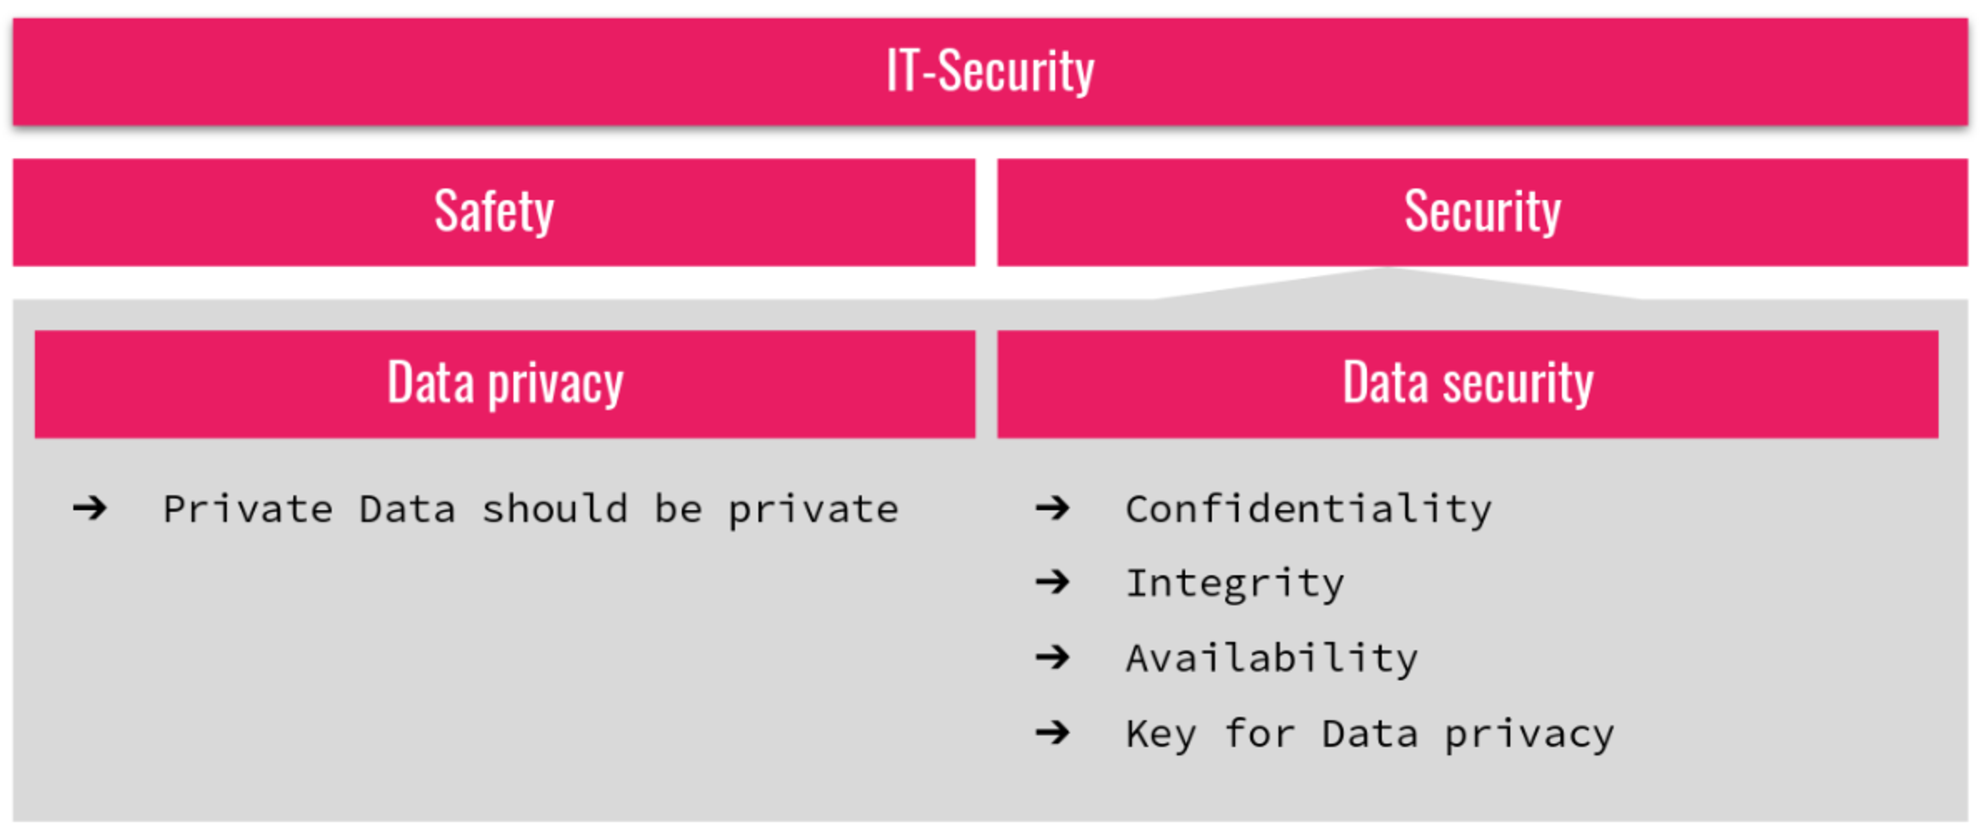
\includegraphics[width=\textwidth, angle=0]{img/it_security.pdf}
		\caption{Parts of IT-Security}
	\label{img:part_it_security}
\end{figure}

\subsection{Safety}
\label{chp:intro:sec:definition:ssec:safety}

The main question in safety is: \textit{Does my application what it is supposed to do?}. \\
So it is about functionality and often directly defined by customers or stakeholder. One strategy to avoid problems with safety topics are automated test. For example unit tests and integration test running by a continuous integration (CI). \\
But safety is not the focused topic.

\subsection{Security}
\label{chp:intro:sec:definition:ssec:safety}

Security is about information and data. Like in Fig. \ref{img:part_it_security} it can be split into privacy and security.

\subsubsection{Privacy}
\label{chp:intro:sec:definition:ssec:safety::sss:privacy}

Privacy' subject is to make sure that personal data like age, name or address are accessible only by people who are allowed. \\
Since \hyperref[https://gdpr-info.eu/]{GDPR} came into force, it is not only a ideological question it is also a lawful question. And not fulfill this law can result in very high fines.\\ The goals, to keep private data private, can only get achieved with security. 

\subsubsection{Security}
\label{chp:intro:sec:definition:ssec:safety::sss:security}

Security has three general targets.

\begin{description}
	\item[Confidentiality] is about making sure to restricted the access to a level where only people with the necessary privileges are allowed to see, change or delete these data.
	
	\item[Integrity] makes sure that every unauthorized change can be detected and changes are verifiable.
	
	\item[Availability] Means that the information should be always available to the user.
\end{description} 

But there are also some more specific target. These does not fit in every use case.

\begin{description}
	\item[Authenticity] aims on reliability. It should be clear that a message comes from the specific sender.
	
	\item[Anonymity] In some cases it should not be possible to connect a network package to a specific person.
\end{description} 

In a lot of cases it is a trade of between these targets. In this case it should be clear why and what it means to not fulfill the target to 100\%.

\newpage
\section{Motivation}
\label{chp:intro:sec:motivation}

Mobile devices get used for a lot of topics. Manage contact, doing phone calls and messaging are only the simplest examples. Nowadays the smartphone is used for nearly everything and became a personal assistant. That means a lot of personal data are stored on the device. Just to mention some of these data:

\begin{itemize}
	\item Identities, for social media but also for credit/customer cards or online banking.
	\item Histories, like browser history or location history
	\item Payments
	\item Location
\end{itemize}

Implementing secure mobile applications can be more difficult than for a regular desktop environment because the user wants a simpler UI and an easy and fast access to their data. So it should be avoided to ask for long inputs or complicated authentication methods.\\
\\
A further difference to the desktop environment is the mobility of these devices. Because of that an smartphone can easily get in the wrong hands. And the connectivity of these devices is higher since they support nearly every modern interface, which can be wired but in the most time is wireless. All these interfaces open a new attack vector, which can be used to get some data or control over the device.\\
\\
But away from the technical background there are more reasons to secure a mobile application. \\
\begin{itemize}
	\item The store provider check their apps for common bugs which can lead to secure gap
	\item Laws like \textit{GDPR} force us to secure user data
	\item Corrupt data inside the app can destroy the user experience
	\item Loosing data can lead to reputational damage
	\item A exploited security issue can cost a lot of money
	\item Your own standards
\end{itemize}



	\chapter{Topics to be aware of}
\label{chp:howto}

\section{Permissions}
\label{chp:howto:sec:permissions}

As the Android OS is built on top of the Linux Kernel it also comes with the permission approach of Linux. This way an application can only access a limited range of system resources by default and every access to a resource is managed by the OS.
To get more access than the standard provided by the basic sandbox, an application must define the resources it wants to have access to in its manifest. The user gets asked to grant these permissions the first time an app wants the access. This gets saved to the device for later usage and the user doesn't have to grant it again.
Like in Linux the permission model is a user based model and as every application is its own user every application has its own permissions. This also isolates the user resources from one another. In addition every application has to explicitly define which resources it shares with other applications.
A good way of requesting permissions is to minimize the number of requested permissions. Simply because if an app can't do more than it should, unexpected situations won't arise. So if a permission is not required it should not be requested.
Also self created permissions should be as few as possible and rather system defined ones should be used as while granting the permissions a user could get confused by a big list of unknown permissions.

\section{Networking}
\label{chp:howto:sec:networking}

Networking with any device is always risky just because of the fact, that the data that has to be transmitted is potentially private data of the user. Any loss or "publication" of this data can harm the user and/or the trust a user has in the application. The highest endeavour should always be to keep user data secure at all times. For this reason it is important to use secure connections to any network an app wants to send data to or receive from. 
The key to secure network traffic is to use appropriate protocols for the connections. For trivial example would be to use HTTPS over HTTP whenever the server provides it.
On a mobile device any network connection covers an additional possible security threat, as it is frequently connected to unsecure networks via Wi-Fi. Here the threat is first that the network itself could be unsecure and second it is not known which other users are in the network and possibly have bad intentions.
Another point is that some developer tend to use localhost ports for sending data over Inter Process Communication (IPC). This is not a good approach as these interfaces are accessible by other applications on the device and so the data could be read by the wrong process. The way to solve this is to use IPC mechanisms provided by android.
	\chapter{Example}
\label{chp:example}

This example is about Google and Apple Pay. It explains how these two paying applications work and why it is done how it is done. \\
Before diving into the algorithm behind the paying methods, some terms should be explained.

\begin{description}
	\item [Payment Networks] are credit institutions which managing credit cards and the transfer from money. But also Paypal and VisaCheckout are payment Networks.
	\item [Token Service Provider] are providing a very secure environment to map credit card information to individual token. \cite{token-service-provider}
	\item [Secure Enclave] is the build in security chip in Apple devices. All keys are stored in here.
	\item [Secure Element] is also apple specific and is paired with the Secure Enclave via hardware in the factory. It is located in the NFC-Chip to emulate the credit card.
\end{description}

Apple Pay and Google Pay are similar but different in detail. Both have four main steps.

\begin{enumerate}
	\item Adding a card
	\item Initiate
	\item Authorize
	\item Finish
\end{enumerate}

\newpage

\section{Google Pay}
\label{chp:example:sec:googlePay}

Google Pay is using the process of tokenization \cite{tokenization} like a lot other mobile payment application and is standardized together with card issuer and token service provider (TSP).\\
\begin{figure}[h!]
	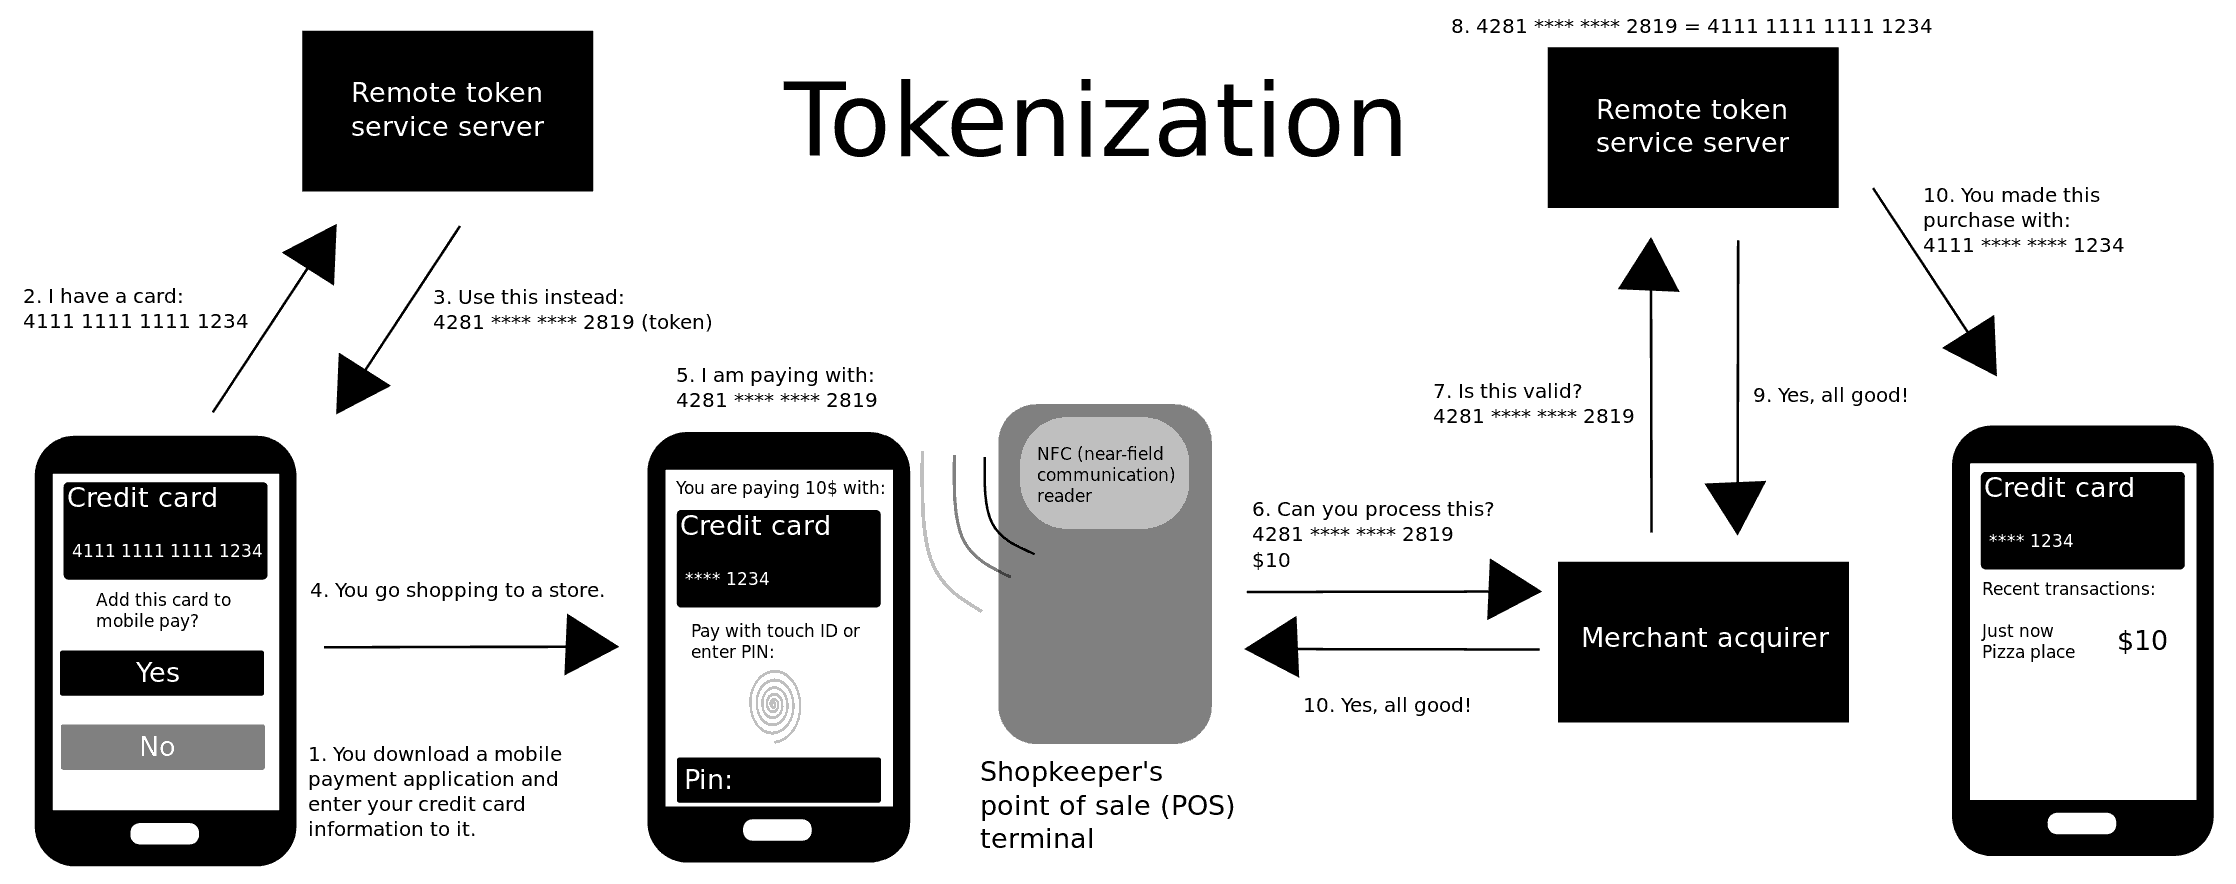
\includegraphics[width=\textwidth, angle=0]{How_mobile_payment_tokenization_works.png}
	\caption{Mobile payment tokenization}
	\label{img:mobile_payment_tokenization}
\end{figure}

\subsection{Adding a card}
\label{chp:example:sec:googlePay:ssec:addingACard}

After downloading the payment app (Fig. \ref{img:mobile_payment_tokenization} Step 1) the user gives the card number. In the background the app ask for a token to represent the card. (Fig. \ref{img:mobile_payment_tokenization} Step 2 and 3)\\
This token, provided from a TSP, is stored at the device and encrypted with a single or limited used key provided from the Payment Network. \\
This is an elegant way to not safe user data on the device. Security of the token is finally guaranteed by encryption. So this step applies two principles of security. 

\subsection{Initiate payment}
\label{chp:example:sec:googlePay:ssec:initiate}

The customers taps their device on a NFC Terminal (Fig. \ref{img:mobile_payment_tokenization} Step 4). With this action the application start transmitting the token, a token expire date and the cryptogram (Fig. \ref{img:mobile_payment_tokenization} Step 5). The cryptogram is generated by the token, timestamp and an Application Transaction Counter which is increased at every transaction and prevent the multiple use of one message.\\
This is a good example how appropriate protocols can be a secure way to communicate even if everybody could listen.\\

\subsection{Authorize}
\label{chp:example:sec:googlePay:ssec:authorize}

The merchant receive the message from NFC terminal and sends all information including the price to his card network (Fig. \ref{img:mobile_payment_tokenization} Step 6 and 7). The card network validates the cryptogram with help of TSP and matches the token to the real card number (Fig. \ref{img:mobile_payment_tokenization} Step 8).
\\
This step also fulfills one principle of security - validation.

\subsection{Finish}
\label{chp:example:sec:googlePay:ssec:finish}

Billing details get decrypted and the acquiring bank completes the transaction with customers bank Merchant and customer get information about validation (Fig. \ref{img:mobile_payment_tokenization} Step 9 and 10).\\ All with appropriated protocols. 
  

	% references
	\bibliographystyle{unsrtdin}
	\bibliography{bib/literature}

\end{document}
